\documentclass[tikz,border=8pt]{standalone}
% Shared look for every TikZ diagram. Load with \input{../../tools/tikz-style.tex}
\usepackage[T1]{fontenc}
\usepackage{lmodern}
\renewcommand{\sfdefault}{lmr}  % diagrams use the same serif as the text
\usetikzlibrary{arrows.meta, positioning, shapes.geometric, calc, fit, backgrounds}
\definecolor{cblue}{HTML}{4C78A8}
\definecolor{corange}{HTML}{F58518}
\definecolor{cgreen}{HTML}{54A24B}
\definecolor{cred}{HTML}{E45756}
\definecolor{cpurple}{HTML}{B279A2}
\definecolor{cgrey}{HTML}{6B6B6B}
\tikzset{
  every picture/.style={font=\sffamily, line width=1.2pt},
  box/.style={draw=#1, fill=#1!12, rounded corners=4pt, align=center, inner sep=7pt, minimum height=1.1cm},
  box/.default=cgrey,
  arrow/.style={-{Stealth[length=3mm]}, draw=cgrey, line width=1.4pt},
  title/.style={font=\sffamily\bfseries\Large},
  note/.style={font=\sffamily\small, text=cgrey, align=center},
}
\AtBeginDocument{\hyphenpenalty=10000 \exhyphenpenalty=10000}

% A differential-drive robot turning left about its turning point. Speeds grow with distance: v = omega R,
% v_R = omega (R + L/2), v_L = omega (R - L/2). Drawn with R = 0.5, L = 0.2, omega = 1 (v_R = 0.6, v = 0.5, v_L = 0.4).
\begin{document}
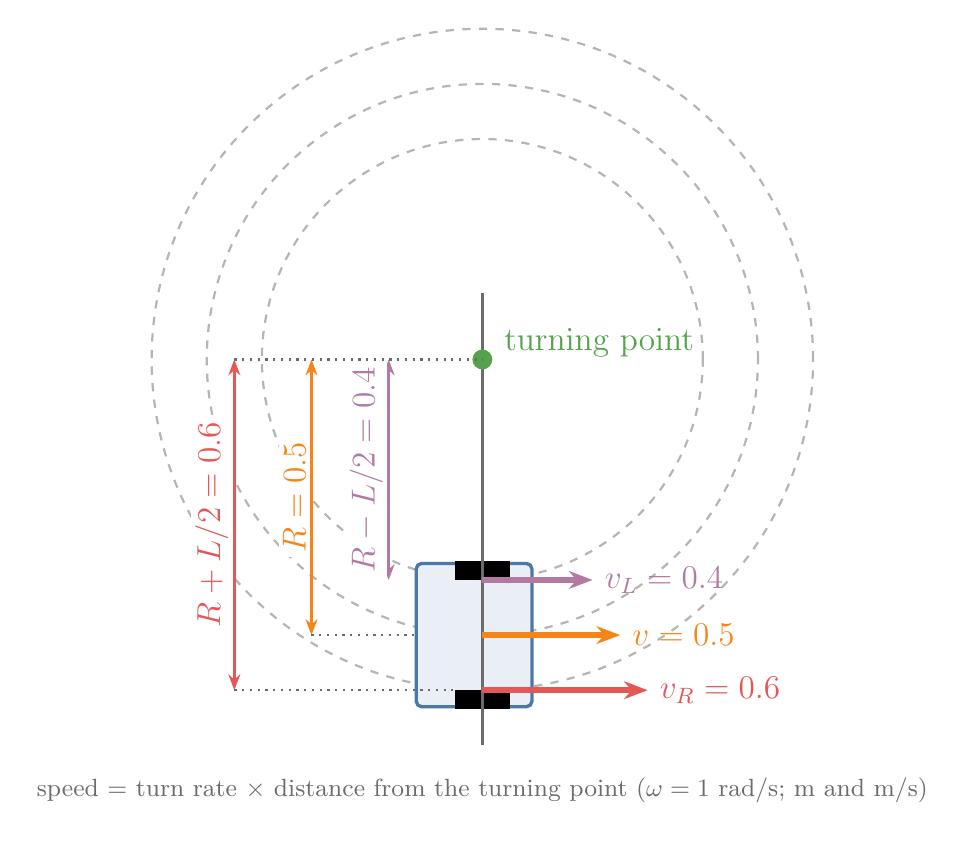
\begin{tikzpicture}[scale=7, every node/.append style={font=\large}]
  \coordinate (C) at (0,0.5);       % turning point
  \draw[cgrey!50, dashed, line width=0.8pt] (0,0.5) circle (0.6);
  \draw[cgrey!50, dashed, line width=0.8pt] (0,0.5) circle (0.5);
  \draw[cgrey!50, dashed, line width=0.8pt] (0,0.5) circle (0.4);
  % robot at the bottom of the circles, facing +x
  \draw[cblue, fill=cblue!12, rounded corners=2pt] (-0.12,-0.13) rectangle (0.09,0.13);
  \fill[black] (-0.05,0.1) rectangle (0.05,0.135);     % left wheel at y = +0.1
  \fill[black] (-0.05,-0.135) rectangle (0.05,-0.1);   % right wheel at y = -0.1
  % axle line through the turning point
  \draw[cgrey, line width=1pt] (0,-0.2) -- (0,0.62);
  \fill[cgreen] (C) circle (0.018);
  \node[cgreen, right] at (0.02,0.53) {turning point};
  % velocity arrows (length = speed x 0.5)
  \draw[-{Stealth[length=3mm]}, cred, line width=2.2pt] (0,-0.1) -- (0.30,-0.1) node[right] {$v_R = 0.6$};
  \draw[-{Stealth[length=3mm]}, corange, line width=2.2pt] (0,0) -- (0.25,0) node[right] {$v = 0.5$};
  \draw[-{Stealth[length=3mm]}, cpurple, line width=2.2pt] (0,0.1) -- (0.20,0.1) node[right] {$v_L = 0.4$};
  % distances, labels written along each arrow
  \draw[{Stealth[length=2mm]}-{Stealth[length=2mm]}, cpurple, line width=1.2pt] (-0.17,0.1) -- (-0.17,0.5) node[midway, sloped, above, fill=white, inner sep=1.5pt] {$R - L/2 = 0.4$};
  \draw[{Stealth[length=2mm]}-{Stealth[length=2mm]}, corange, line width=1.2pt] (-0.31,0) -- (-0.31,0.5) node[midway, sloped, above, fill=white, inner sep=1.5pt] {$R = 0.5$};
  \draw[{Stealth[length=2mm]}-{Stealth[length=2mm]}, cred, line width=1.2pt] (-0.45,-0.1) -- (-0.45,0.5) node[midway, sloped, above, fill=white, inner sep=1.5pt] {$R + L/2 = 0.6$};
  \draw[cgrey, dotted, line width=0.8pt] (-0.45,0.5) -- (0,0.5);
  \draw[cgrey, dotted, line width=0.8pt] (-0.45,-0.1) -- (-0.05,-0.1);
  \draw[cgrey, dotted, line width=0.8pt] (-0.31,0) -- (-0.12,0);
  \node[note, anchor=north] at (0,-0.24) {speed $=$ turn rate $\times$ distance from the turning point ($\omega = 1$ rad/s; m and m/s)};
\end{tikzpicture}
\end{document}
